%%%%%%%%%%%%%%%%%%%% author.tex %%%%%%%%%%%%%%%%%%%%%%%%%%%%%%%%%%%
%
% sample root file for your "contribution" to a contributed volume
%
% Use this file as a template for your own input.
%
%%%%%%%%%%%%%%%% Springer %%%%%%%%%%%%%%%%%%%%%%%%%%%%%%%%%%


% RECOMMENDED %%%%%%%%%%%%%%%%%%%%%%%%%%%%%%%%%%%%%%%%%%%%%%%%%%%
\documentclass[graybox,vecphys]{svmult}

% choose options for [] as required from the list
% in the Reference Guide

\usepackage{type1cm}        % activate if the above 3 fonts are
                            % not available on your system
%
\usepackage{makeidx}         % allows index generation
\usepackage[dvipdfmx]{graphicx}
%\usepackage{graphicx}        % standard LaTeX graphics tool
%                             % when including figure files
\usepackage{multicol}        % used for the two-column index
\usepackage[bottom]{footmisc}% places footnotes at page botto

%\usepackage{vecphys}

\usepackage{newtxtext}       % 
\usepackage{newtxmath}       % selects Times Roman as basic font

\usepackage{url}

% see the list of further useful packages
% in the Reference Guide

\makeindex             % used for the subject index
                       % please use the style svind.ist with
                       % your makeindex program

%%%%%%%%%%%%%%%%%%%%%%%%%%%%%%%%%%%%%%%%%%%%%%%%%%%%%%%%%%%%%%%%%%%%%%%%%%%%%%%%%%%%%%%%%

\begin{document}

\title*{Parallelization of Atomic Image Reconstruction
  from {X-ray} Fluorescence Holograms with {XcalableMP}}
\titlerunning{Parallelization of Atomic Image Reconstruction from Holograms}
% Use \titlerunning{Short Title} for an abbreviated version of
% your contribution title if the original one is too long
\author{Atsushi Kubota, Tomohiro Matsushita and Naohisa Happo}
% Use \authorrunning{Short Title} for an abbreviated version of
% your contribution title if the original one is too long
\institute{Atsushi Kubota and Naohisa Happo \at Hiroshima City University, Hiroshima 731-3194 Japan, \email{\{kubota,happo\}@hiroshiam-cu.ac.jp}
\and Tomohiro Matsushita \at Japan Synchrotron Radiation Research Institute (JASRI), SPring-8, Sayo, Hyogo 679-5198 Japan \email{matusita@spring8.or.jp}}
%
% Use the package "url.sty" to avoid
% problems with special characters
% used in your e-mail or web address
%
\maketitle

\abstract*{
    X-ray fluorescence holography is a three-dimensional middle range
  local structure analysis method, which can provide three-dimensional
  atomic images around specific elements within a radius of a few
  nanometers. Three-dimensional atomic images are reconstructed by
  applying discrete Fourier transform (DFT) to hologram
  data. Presently, it takes long time to process this DFT. In this
  study, the DFT program is parallelized by using a parallel
  programming language XcalableMP. The DFT process, whose input is 21
  holograms data of 179 {$\times$} 360 points and output is a
  three-dimensional atomic image of {$192^3$} points, is executed on
  PC cluster which consists of 8 nodes of Intel Xeon X5660 processors
  and 96 cores in total and we confirmed that the parallelized DFT
  execution is 94 times faster than the sequential execution.}


\abstract{    X-ray fluorescence holography is a three-dimensional middle range
  local structure analysis method, which can provide three-dimensional
  atomic images around specific elements within a radius of a few
  nanometers. Three-dimensional atomic images are reconstructed by
  applying discrete Fourier transform (DFT) to hologram
  data. Presently, it takes long time to process this DFT. In this
  study, the DFT program is parallelized by using a parallel
  programming language XcalableMP. The DFT process, whose input is 21
  holograms data of 179 {$\times$} 360 points and output is a
  three-dimensional atomic image of {$192^3$} points, is executed on
  PC cluster which consists of 8 nodes of Intel Xeon X5660 processors
  and 96 cores in total and we confirmed that the parallelized DFT
  execution is 94 times faster than the sequential execution.}

\section{Introduction}
\label{sec:1}
%Use the template \emph{chapter.tex} together with the document class SVMono (monograph-type books) or SVMult (edited books) to style the various elements of your chapter content.

%Instead of simply listing headings of different levels we recommend to let every heading be followed by at least a short passage of text.  Further on please use the \LaTeX\ automatism for all your cross-references and citations. And please note that the first line of text that follows a heading is not indented, whereas the first lines of all subsequent paragraphs are.

X-ray fluorescence holography (XFH) is a three-dimensional middle
range local structure analysis method, which can proved 3D atomic
images around specific elements within a radius of a few
nanometers\cite{Hayashi-JSSRR2013-Eng}.  Compared to other method such
as X-ray diffraction, which has been widely used for structure
analysis of crystals and other materials, XFH is more sensitive to
atomic fluctuations, and therefore it is useful for characterization
of local lattice distortions.

In the XFH method, hologram data are obtained by experiments done at
large synchrotron facilities such as SPring-8 and KEK-PF.
Three-dimensional atomic images are reconstructed from the obtained
holograms by Barton's method\cite{Barton-PRL1988,Barton-PRL1991}.  In
Barton's method, it takes long time to reconstruct the atomic
images from the obtained holograms.
%by applying discrete Fourier transform (DFT).

In distributed memory computing environment such as PC clusters and
supercomputers, hybrid parallelization is widely used by describing
inter- and intra- node parallelism with Message-Passing Interface
(MPI)~\cite{MPI3_1} and OpenMP~\cite{OpenMP5} respectively. However, it
is pointed out that MPI programs tend to be complicated and error-prone.
% tedeous
Therefore, in order to improve productivity of parallel programming, a
variety of parallel programming languages, language extentions and
libraries have been proposed. Some examples of them are High
Performance Fortran (HPF)~\cite{HPF}, CoArray adopted
in Fortran2008, UPC~\cite{UPC2019}, which is based on C language, and
XcalableMP~\cite{XcalableMP1_4}, in which distribution of data and
parallelization of loops are specified by directives. New parallel
programming languages such as X10~\cite{X10_2_6_2} and Chapel~\cite{Chapel2015}
are also proposed.

We adopted a hybrid parallel programming approach, in which inter- and
intra- node parallelism are described in XcalableMP and OpenMP
respectively to parallelize the existing atomic image reconstruction
program by Barton's method written in C language because it
can be parallelized with small amount of modification.

In the rest of this chapter, X-ray fluorescence holography
and reconstruction of atomic images are explained in Section \ref{sec:xfh}.
Parallelization of atomic image reconstruction is explained
in Section \ref{sec:parallelization} and its performance results are
shown in Section \ref{sec:results}. Finally, conluding remarks are
given in Section \ref{sec:conclusion}


\section{X-ray Fluorescence Holography}\label{sec:xfh}

There are two modes in XFH, namely, the normal mode and the inverse
mode.  In this chapter, we focus on the inverse mode because it is
mainly used in experiments of XFH recently. Please refer to the
literatures such as \cite{Hayashi-JSSRR2013-Eng} in details.

In the inverse mode, the angle of a sample material to the incident
X-ray is varied as shown in Fig.~\ref{fig:inverse} and intensity
of X-ray fluorescence emitted from atoms in the sample is measured
by the detector.

\begin{figure}[tb]
%  \sidecaption
  \begin{center}
%  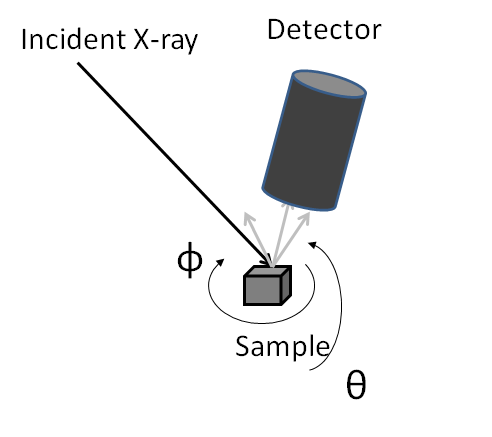
\includegraphics[width=6cm]{inverse.png}
  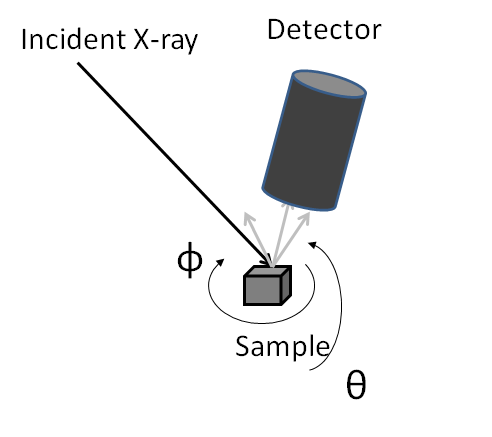
\includegraphics[width=10cm]{inverse.png}
  \caption{Inverse Mode of XFH}\label{fig:inverse}
  \end{center}
\end{figure}
%\caption{If the width of the figure is less than 7.8 cm use the \texttt{sidecapion} command to flush the caption on the left side of the page. If the figure is positioned at the top of the page, align the sidecaption with the top of the figure -- to achieve this you simply need to use the optional argument \texttt{[t]} with the \texttt{sidecaption} command}

As shown in Fig.~\ref{fig:inversemode}, the incident X-ray approaching
atom A and another incident X-ray also approaching atom A after
scattered by atom B form a constant wave of X-ray around atom A.
The pattern of the constant wave from atom A varies according to
the angle of the incident X-ray and resulted in the variation of
the intensity of the X-ray fluorescence from atom A. Experimental
data obtained by measuring the intensity of X-ray fluorescence
make a hologram of the atomic image.

\begin{figure}[bt]
  \begin{center}
    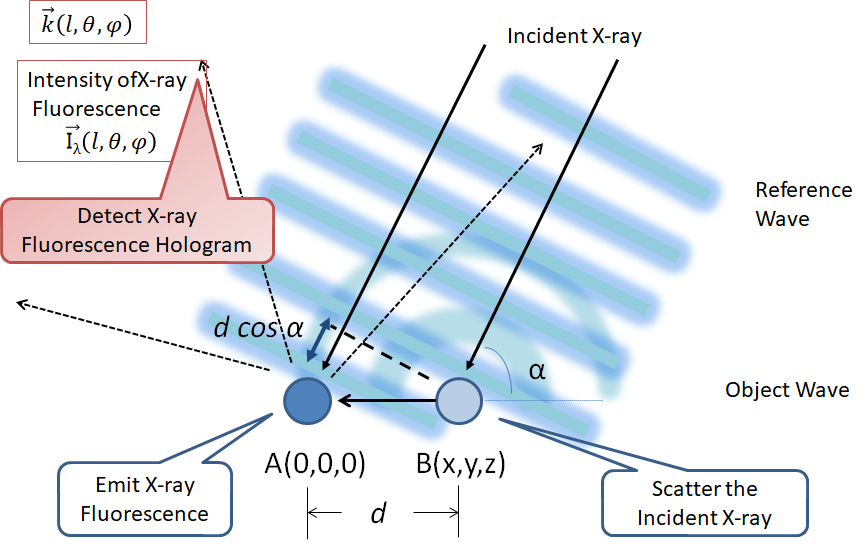
\includegraphics[width=10cm]{inversemode_alpha.png}
    \caption{Difference of Optical Path Length in Inverse Mode}\label{fig:inversemode}
  \end{center}
\end{figure}

Incident X-ray wave approaching atom A directly corresponds to
reference wave of ordinary hologram and incident X-ray wave
approaching atom A after scattered by atom B corresponds to
object wave.


\subsection{Reconstruction of Atomic Images}
\label{subsec:reconst}

When the intensity $I_{\lambda}(l,\theta,\phi)$ measured at polar
coordinate system $\vec{k}(l,\theta,\phi)$ on a hologram on a sphere
by incident X-ray of wave length $\lambda$, the position of an atom
in the sample can be calculated as follows.

Suppose atom A and B are located at the origin and $\vec{r}(x,y,z)$
in the sample, the atomic image of atom b can be reconstructed by
calculation similar to three-dimensional descrete Fourier Transform.
In atomic images reconstructed from holograms obtained by several wave
lengths, real atomic images are enhanced and, at the same time, ghost
images are reduced\cite{Hayashi-JSSRR2013-Eng}.  In order to reduce
the processing time , atomic images are reconstructed from the
hologram on the sphere of radius $l$ as shown in Eq.~(\ref{eqn:dft3d}):

\begin{equation}\label{eqn:dft3d}
  \chi(x,y,z) = \sum_{\theta} \sum_{\phi} \sum_{\lambda}
  - I_{\lambda}(\theta,\phi) \exp({i2 \pi (|\vec{r}| - \vec{k}\vec{r}) /
    \lambda}) \sin\theta
\end{equation}
%% \begin{eqnarray}\label{eqn:dft3d}
%%   \chi(x,y,z) & = & \sum_{\theta} \sum_{\phi} \sum_{\lambda}
%%   - I_{\lambda}(\theta,\phi) \exp({i2 \pi (|\vec{r}| - \vec{k}\vec{r}) /
%%     \lambda}) \nonumber\\
%%               & {\times} & \sin\theta
%% \end{eqnarray}

%% %
%% however, for multiline equations we recommend to use the \verb|eqnarray| environment\footnote{In physics texts please activate the class option \texttt{vecphys} to depict your vectors in \textbf{\itshape boldface-italic} type - as is customary for a wide range of physical subjects}.
%% \begin{eqnarray}
%% \left|\nabla U_{\alpha}^{\mu}(y)\right| &\le&\frac1{d-\alpha}\int
%% \left|\nabla\frac1{|\xi-y|^{d-\alpha}}\right|\,d\mu(\xi) =
%% \int \frac1{|\xi-y|^{d-\alpha+1}} \,d\mu(\xi)  \\
%% &=&(d-\alpha+1) \int\limits_{d(y)}^\infty
%% \frac{\mu(B(y,r))}{r^{d-\alpha+2}}\,dr \le (d-\alpha+1)
%% \int\limits_{d(y)}^\infty \frac{r^{d-\alpha}}{r^{d-\alpha+2}}\,dr
%% \label{eq:01}
%% \end{eqnarray}

The input data are stored in double precision floating point number
format. Coordinate on the sphere is represented in the polar coordinate
system ranging from $\theta$ = 1 degree to 179 degree and from $phi$ =
0 degree to 359 degree by 1 degree grid on each angle. The output data
are grid points values on the rectangular coordinate
system ranging from -10 to 10.0 angstrom by 0.1 angstrom grid on each
axis. The complex numbers at grid points
calculated by the reconstruction are stored in the output file.

192 grid points are laid on each axis on the rectangular coordinate system
ranging from -9.6 to 9.6 angstrom by 0.1 angstrom grid
in order to parallelize the reconstruction easily on PC cluster,
it is explained in detail in Sect.~\ref{sec:results}.


Because the grid points of input data are located on the polar coordinate
system and, on the other hand, those of ouput data are on
the rectangular coordinate system, it is difficult to apply the fast
Fourier transform (FFT) algorithm to DFT and it takes long time to
calculate DFT.

We estimate that it may take a few days to reconstruct the
three-dimensional atomic images from holograms measured by
experiments. Because crystal structure of sample and its lattice
constant are already known by other methods, in order to reduce the
time required for reconstruct atomic images for crystal with a certain
lattice constant, for example 2 angstrom, three-dimensional atomic
images are estimated with several two-dimensional atomic images on x-y
planes at z = -4, -2, 0, 2, 4 angstrom.  If needed, atomic images at z
= -1.9 and 2.1 angstrom are reconstructed to analyze atomic
fluctuations and lattice distortions.

Thus, it takes long time to analyze the crystal structure because
reconstruction of two-dimensional atomic images and observation of the
atomic images repeatedly.

\subsection{Analysis Procedure of XFH}\label{sec:xfh_analysis}
In XFH, experimental data are analyzed in the following procedure.
The most time consuming step is reconstruction while pre- and post- steps
are also needed.

\begin{enumerate}
\item experiment
\item removal of background waves
\item completion of sphere data
\item reconstruction of atomic images and
\item display of them
\end{enumerate}

\begin{figure}[t]
  \begin{center}
    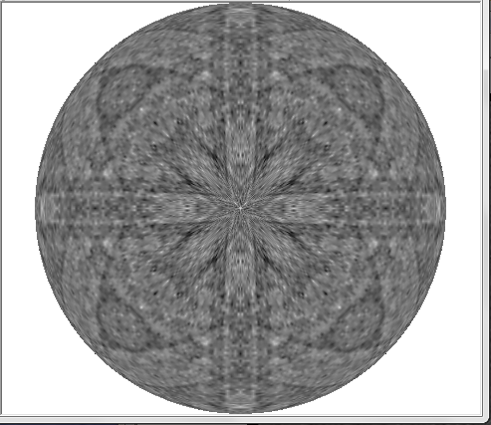
\includegraphics[width=8cm]{sphere18500ev.png}
    \caption{An example hologram obtained by an experiment}\label{fig:hologram}
  \end{center}
\end{figure}

Because it is known that low frequency noise called backgroud wave is
included in hologram data obtained by XFH experiments, the noise is
removed before reconstruction.

In the experiment, the intensity of X-ray fluorescence emitted from
sample is measured while it is slanted from $\theta$ = 0 to 75 degree
and rotated from $\phi$ = 0 to 360 degree at each $\theta$ in
Fig.~\ref{fig:inverse}.  For $\theta$ $>$ 75 degree, the meaningful
intensity is not measured because the surface of the sample and the
incident X-ray are nearly parallel. By making use of symmetry of
crystal structure of the sample, the hologram data on the sphere
ranging from $\theta$ = 0 to 180 degree are completed.  An example of
hologram on the sphere shown in Fig.~\ref{fig:hologram} is obtained by
their pre-processes such as removal of background waves and completion
of sphere data.

The values on grid points of the reconstructed atomic images are
merely values proportional to existence probability
of atom at each grid point on the x-y-z rectangular coordinate system.
For a grid point, the value of low existence probability is noise and
its atom image is not displayed if the value is less than threshold value
and reconstructed images are displayed as shown in Fig.~\ref{fig:ccto}.

\begin{figure}[t]
  \begin{center}
    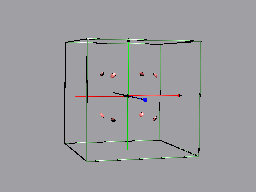
\includegraphics[width=8cm]{CCTO_Cu_9200_3d.png}
    \caption{An example of reconstructed three-dimensional atom images}
      \label{fig:ccto}
  \end{center}
\end{figure}

\section{Parallelization}\label{sec:parallelization}
As pointed out in Sect.~\ref{sec:xfh}, it is an issue 
that it takes long time to analyze the cyristal structure because
reconstruction of two-dimensional atomic images and observation
of the images are repeated several times.
We therefore try to improve the reconstruction of three-dimensional
atomic images by parallelizing DFT with parallel programming language
XcalableMP and parallel API OpenMP on multi-node PC clusters.

OpenMP~\cite{OpenMP5} is a parallel programming API which enables
parallelization by inserting directives in sequential programs.  It
enables parallelization of loops with data parallelism easily and high
performance on shared-memory machines can be achieved. Similar to
OpenMP, XcalableMP~\cite{XcalableMP1_4} is a parallel programming language
which also enables parallelization by inserting directives in
sequential programs. Data distribution among distributed-memory
computing environment such as multi-node PC clusters and
supercomputers can be specified by inserting directives. Both OpenMP and
XcalableMP are designed so that directives related to parallelization
are ignored when the program is compiled to a sequential
executable. Thus both sequential and parallel programs are maintained
in one common source code. In addition, XcalableMP and OpenMP can be
used at the same time for hybrid inter- and intra- node
parallelization.

In this section, hybrid parallelization of reconstruction in two
steps as follows:
\begin{enumerate}
\item parallelization of reconstruction of two-dimensional atomic images
  by OpenMP on single PC node and
\item parallelization of reconstruction of three-dimensional atomic images
  by XcalableMP and OpenMP on multi-nodes.
\end{enumerate}

\subsection{Paralleization of Reconstruction of Two-dimensional Atomic Images by OpenMP}\label{sec:two_d_para}
Presently, according to the Eq.~(\ref{eqn:dft3d}), in the loop of
reconstruction of two-dimensional atomic images at certain z on x-y
plane, five loops of $x$, $y$, $\theta$, $\phi$ and $\lambda$ are nested
from outer to inner loop. In this chapter, $\theta$ loop denotes
the loop which accesses contiguous elements in a dimension of array $\theta$
for short.

The strategy of optimization and parallelization of two-dimensional
reconstruction is as follows:
\begin{enumerate}
\item Replace trigonometric function calls with arrey references,
\item Apply loop interchange and
\item Choose a loop to be parallelized.
\end{enumerate}
These optimizatin and parallelization are explained below.

% x and y loops can be straightforwardly parallelized.
% theta, phi and lambda loops are reduction type parallelizable loops.

In reconstruction of two-dimensional atomic images, some calls of
trigonometric functions such as sin and cos in nested loops are
replaced with references of arrays. The values of the trigonometric
functions are stored in the arrays before entering the nested loops.
% some calls of trigonometric functions remain in the loop nest

In this study, this nested loop is interchanged to $\lambda$, $x$, $y$,
$\theta$ and $\phi$ from outer to inner loop to improve the cache
hit ratio. The size of the three-dimensional input array whose
dimensions are $\lambda$, $\theta$, and $\phi$ is about 10MB and
may not be stored on the secondary cache. In order to improve
the cache hit ratio, when $\lambda$ is fixed at the most outer loop, 
500KB data of the input array for a $\lambda$ are stored on the cache
and accessed repeatedly in the nested loop of $x$, $y$, $\theta$ and $\phi$.
In the original loop nests, the index range of the inner-most $lambda$
loop is at most 20. After interchanging loops, the index range of the
inner-most $phi$ is 360 and it is expected that SIMD instructions in
general purpose processors such as Intel AVX can be applied to the
inner-most loop.

After these optimizations, the $x$ loop in the nested loops is
parallelized by OpenMP directive so that the performance of
reconstruction of two-dimensional atomic images is improved.

\subsection{Parallelization of Reconstruction of Three-dimensional Atomic Images by XcalableMP}\label{sec:three_d_para}
In reconstruction of three-dimensional atomic images, according to the
Eq.~(\ref{eqn:dft3d}), by extending the optimized and parallelized
nested loop of reconstruction of two-dimensional atomic images as
described in Subsect.~\ref{sec:two_d_para}, the six loops of $\lambda$, $z$,
$x$, $y$, $\theta$ and $\phi$ are nested from outer to inner loop.
Similar to the two-dimensional loop, the values of some trigonometric
functions are calculated in advance before entering the six nested
loop.

Among the six nested loops, the outer $z$ loop and the inner $x$ loop
are parallelized by XcalableMP and OpenMP. In other words, the nested
loops are parallelized among inter-nodes by the $z$ loop level and
also parallelized within each node by the $x$ loop level.  The
parallelized kernel loop of three-dimensional atomic image
reconstruction is shown in Fig.~\ref{fig:kernel_loop}.  Other combinations
of parallelizing $x$, $y$ and $z$ loops are also performed and
discussed in Sect~\ref{sec:results}.

\begin{figure}[tb]
\begin{verbatim}
for (l=0; l<No_Incident; l++) {
  input_hologram(l, Xi);
#pragma xmp loop on t(z)
  for (iz=0; iz<NZ; iz++) {
    z = position(iz);
#pragma omp parallel for private(...)
    for (ix=0; ix<NX; ix++) {
      x = position(ix);
      for (iy=0; iy<NY; iy++) {
        y = position(iy);
        r_norm = norm(x,y,z);
        sum1r = 0.0;
        sum1i = 0.0;
        for (th=1; th<NTHETA; th++) {
          sum2r = 0.0;
          sum2i = 0.0;
          for (phi=0; phi<NPHI; phi++) {
            d = r_norm
              - tab_kx[th][phi]*x
              - tab_ky[th][phi]*y
              - tab_kz[th]*z;
            a = k[l]*d;
            sum2r += Xi[th][phi]*cos(a);
            sum2i += Xi[th][phi]*sin(a);
          } /* end for phi */
          sum1r += sum2r * tab_sin[th];
          sum1i += sum2i * tab_sin[th];
        } /* end for theta */
        Ur_r[z][x][y] += sum1r * wt[l];
        Ur_i[z][x][y] += sum1i * wt[l];
      } /* end for y */
    } /* end for x */
  } /* end for z */
} /* end for l */
\end{verbatim}
\begin{center}
  \caption{Kernel loop of three-dimensional atomic image reconstruction}\label{fig:kernel_loop}
\end{center}
\end{figure}

In this study, $z$ loop is parallelized by XcalableMP directives and
the output arrays are distributed contiguously, namely BLOCK
distribution, among nodes in $z$ dimension as shown in
Fig.~\ref{fig:arrays}.  All of the input data are read on every node
simultaneously and stored replicated. The data of atomic images, which
are distributed among nodes in $z$ dimension, are calculated on each
node, aggregated to one root node as shown in Fig.~\ref{fig:aggregation}
and finally written to the output file on the root node.

\begin{figure}[tb]
\begin{verbatim}
#pragma xmp nodes p(1)
#pragma xmp template t(0:191)
#pragma xmp distribute t(block) onto p

/* input array */
double Xi[NTHETA][NPHI];

/* output arrays */
double Ur_r[NZ][NX][NY];
#pragma xmp align Ur_r[n][*][*] with t(n)
double Ur_i[NZ][NX][NY];
#pragma xmp align Ur_i[n][*][*] with t(n)
double Ur_r1[NZ][NX][NY];
double Ur_i1[NZ][NX][NY];
\end{verbatim}
\begin{center}
  \caption{Input and output arrays and specification of their distribution by XcalableMP directives}\label{fig:arrays}
\end{center}
\end{figure}

\begin{figure}[tb]
\begin{verbatim}
#pragma xmp gmove
Ur_r1[:][:][:] = Ur_r[:][:][:];
#pragma xmp gmove
Ur_i1[:][:][:] = Ur_i[:][:][:];
\end{verbatim}
\begin{center}
  \caption{Aggregation of arrays by XcalableMP}\label{fig:aggregation}
\end{center}
\end{figure}

\section{Performance Evaluation}\label{sec:results}
In this section, we show the performance results of parallel runs
of reconstruction of two-dimensional atomic images parallelized by OpenMP
executed on a single node and reconstruction of three-dimensional atomic images
parallelized by XcalableMP and OpenMP on a multi-node PC cluster.
Comparison of XcalableMP and MPI for multi-node parallelization
with respect to the performance and productivity of programming are
also demonstrated.

The PC cluster consist of eight nodes and each node has two sockets of
six-core Intel Xeon X5660 2.8GHz and 24GB main memory. The nodes are
connected with InfiniBand DDR(4Gbps) and Gigabit Ethernet. The size of
smart cache on Xeon X5660 is 12MB. The program is compiled with XcalableMP
1.2.2 and Intel Compiler 18.0.1 with -O3 -XHOST optimization option.

\subsection{Performance Results of Reconstruction of Two-dimensional Atomic Images}
The program of reconstruction of two-dimensional atomic images is
executed on a single node of the PC cluster. The input data are
obtained in an experiment in which lead zirconate titanate (PZT) is
used as a sample in the experiment and 21 types of incident X-rays are
entered to the sample while varying angles ranging from $\theta$ = 1
to 179 degree and from $\phi$ = 0 to 359 degree. The output is an
two-dimensional array [x][y] = [192][192] for a certain $z$.

In Table~\ref{tab:reconst2d}, the execution time of the original,
array reference of trigonometric function calls and loop interchange on
one node.  Execution time and speed-up ratio of the program
parallelized by OpenMP with 12 threads on two sockets of six core Xeon
are 75.814 sec. and 12.8 respectively.

Here, let us consider the effect of the loop interchange.
The size of input three-dimensional double precision array ($\lambda$,
$\theta$, $\phi$) is about 10MB. Before the loop interchange, loops $x$
and $y$ are the outer loops and 10MB input data is repeatedly referenced
in the nest of inner three loops $\lambda$, $\theta$ and $\phi$. Because
the size of smart cache is 12MB, it is assumed that the input data are
spilled out of the cache and cache misses are occured frequently.
On the contrary, $\lambda$ loop is placed at the outer-most the loop nests
by the loop interchange and a part of the input data is repeatedly
referenced in the inner loops $\theta$ and $\phi$. This fragement of
the input data is about 500KB and can be stored in the smart cache.

%On the contrary,
%% As discussed in \ref{sec:two_d_para}, 
%% when the $\lambda$ loop is moved to outer most by
%% loop exchange, 500KB input data is repeatedly referenced in the inner
%% nested loop of $\theta$ and $\phi$. Because 500KB input data may be stored
%% on the last level cache.

% It seems that array references and loop exchange have no effect on
% performance improvement, these optimizations are required for better
% parallelized performance

\begin{table}[t]
  \begin{center}
  \caption{Performance Results of Reconstructon of Two-dimensional Atomic Images by OpenMP on Xeon X5660}\label{tab:reconst2d}
  \begin{tabular}{r|r|r|r}\hline\hline
    Original (s) & Array References and    & OpenMP(s) & Speed-up Ratio \\
                & Loop Exchange (s)        & 12 threads &          \\\hline\hline
    972.473     & 914.301                  &     75.814 & 12.8 \\
    \hline
  \end{tabular}
  \end{center}
\end{table}

\subsection{Performance Results of Reconstruction of Three-dimensional Atomic Images}
The reconstruction of three-dimensional atomic images are executed
mainly on the six nested loops of $\lambda$, $z$, $x$, $y$, $\theta$
and $\phi$.

The input and output data are stored in three-dimensional arrays of
[$\lambda$][$\theta$][$\phi$] = [21][179][360] and [z][x][y] =
[192][192][192] respectively. The output array is divided in $z$ dimension
and distributed among nodes on the PC cluster.

The $z$ loop and $x$ loop in the reconstruction program is
parallelized by XcalableMP and OpenMP respectively. The performance
results of parallel execution on the PC cluster are shown in Table~\ref{tab:xmp_z192} and \ref{tab:xmp_z8}.
For the size of output [z][x][y] = [192][192][192],
because the estimation time of the sequential execution is too long,
it is executed when the total number of threads is greater or equal to eight
as shown in Table~\ref{tab:xmp_z192}.
The \#Threads columns of both Table~\ref{tab:xmp_z192} and \ref{tab:xmp_z8}
stand for the total number of threads, which is the product of the number
of nodes and the number threads per node. In addition to the total execution
time, time for reading from the input file, aggregating the atomic images
distributed among nodes, and writing to the output file.

The performance results of reconstruction of only for eight x-y planes
at Z=0,1$\ldots$7 are shown in Table~\ref{tab:xmp_z8}. Because it
takes a few hours in the sequential execution, this reconstruction are
executed with threads ranging from 1 to 96.

The speed-up ratio of reconstruction of atomic images of both 192 and
8 x-y planes are depicted in Fig.~\ref{fig:xmp96}. Both horizontal and
vertical axes are logarithmic scales. The Z8 graph is the speed-up
ratio to the one thread execution in Table~\ref{tab:xmp_z8}. The Z192
graph is the speed-up ratio to the eight thread execution in
Table~\ref{tab:xmp_z192} multiplied by 8. In both lines in
Fig.~\ref{fig:xmp96}, it is confirmed that nearly ideal speed-up is
achieved. The speed-up ratio values at 96 threads for Z8 and Z192 are
94.21 and 94.23 respectively.

Because the sizes of input and output data are small, the ratio of the
file I/O time to the total execution time is very small and the time of
aggregation of distributed data to one root node by gmove construct of
XcalableMP is also very short. Therefore, high performance is achieved
without parallel file I/O.

\begin{table}[t]
  \begin{center}
  \caption{Performance Results for Reconstruction (z:192) Parallelized by XcalableMP}\label{tab:xmp_z192}
  \begin{tabular}{l|r|rrr}\hline\hline
    \#Threads & Execution (s)    & Input (s) & Aggregation (s) & Output (s)\\\hline\hline
    8(8x1)   &  21,683.076 & 0.781  &  0.176 &  9.772 \\
%    12(1x12) &  53,487.572 & 0.576  &  0.000 & 12.967 \\
    48(8x6)  &   3,623.352 & 0.721  &  0.163 &  9.731 \\
    96(8x12) &   1,840.942 & 0.767  &  0.174 &  9.701 \\
    \hline
  \end{tabular}
  \end{center}
\end{table}

\begin{table}[t]
  \begin{center}
  \caption{Performance Results for Reconstruction (z:8) Parallelized by XcalableMP}\label{tab:xmp_z8}
  \begin{tabular}{l|r|rrr}\hline\hline
    \#Threads & Execution (s)    & Input (s) & Aggregation (s) & Output (s)\\\hline\hline
    1(1x1)   &  7,214.325 & 0.745  & 0.007  & 0.301 \\
%    6(1x6)   &  4,131.279 & 0.579  & 0.000  & 0.304 \\
    8(8x1)   &    923.830 & 0.473  & 0.009  & 0.303 \\
    12(1x12) &    603.962 & 0.459  & 0.005  & 0.310 \\
    48(8x6)  &    151.574 & 0.458  & 0.008  & 0.303 \\
    96(8x12) &     76.576 & 0.455  & 0.009  & 0.310 \\
    \hline
  \end{tabular}
  \end{center}
\end{table}

\begin{figure}[t]
  \begin{center}
  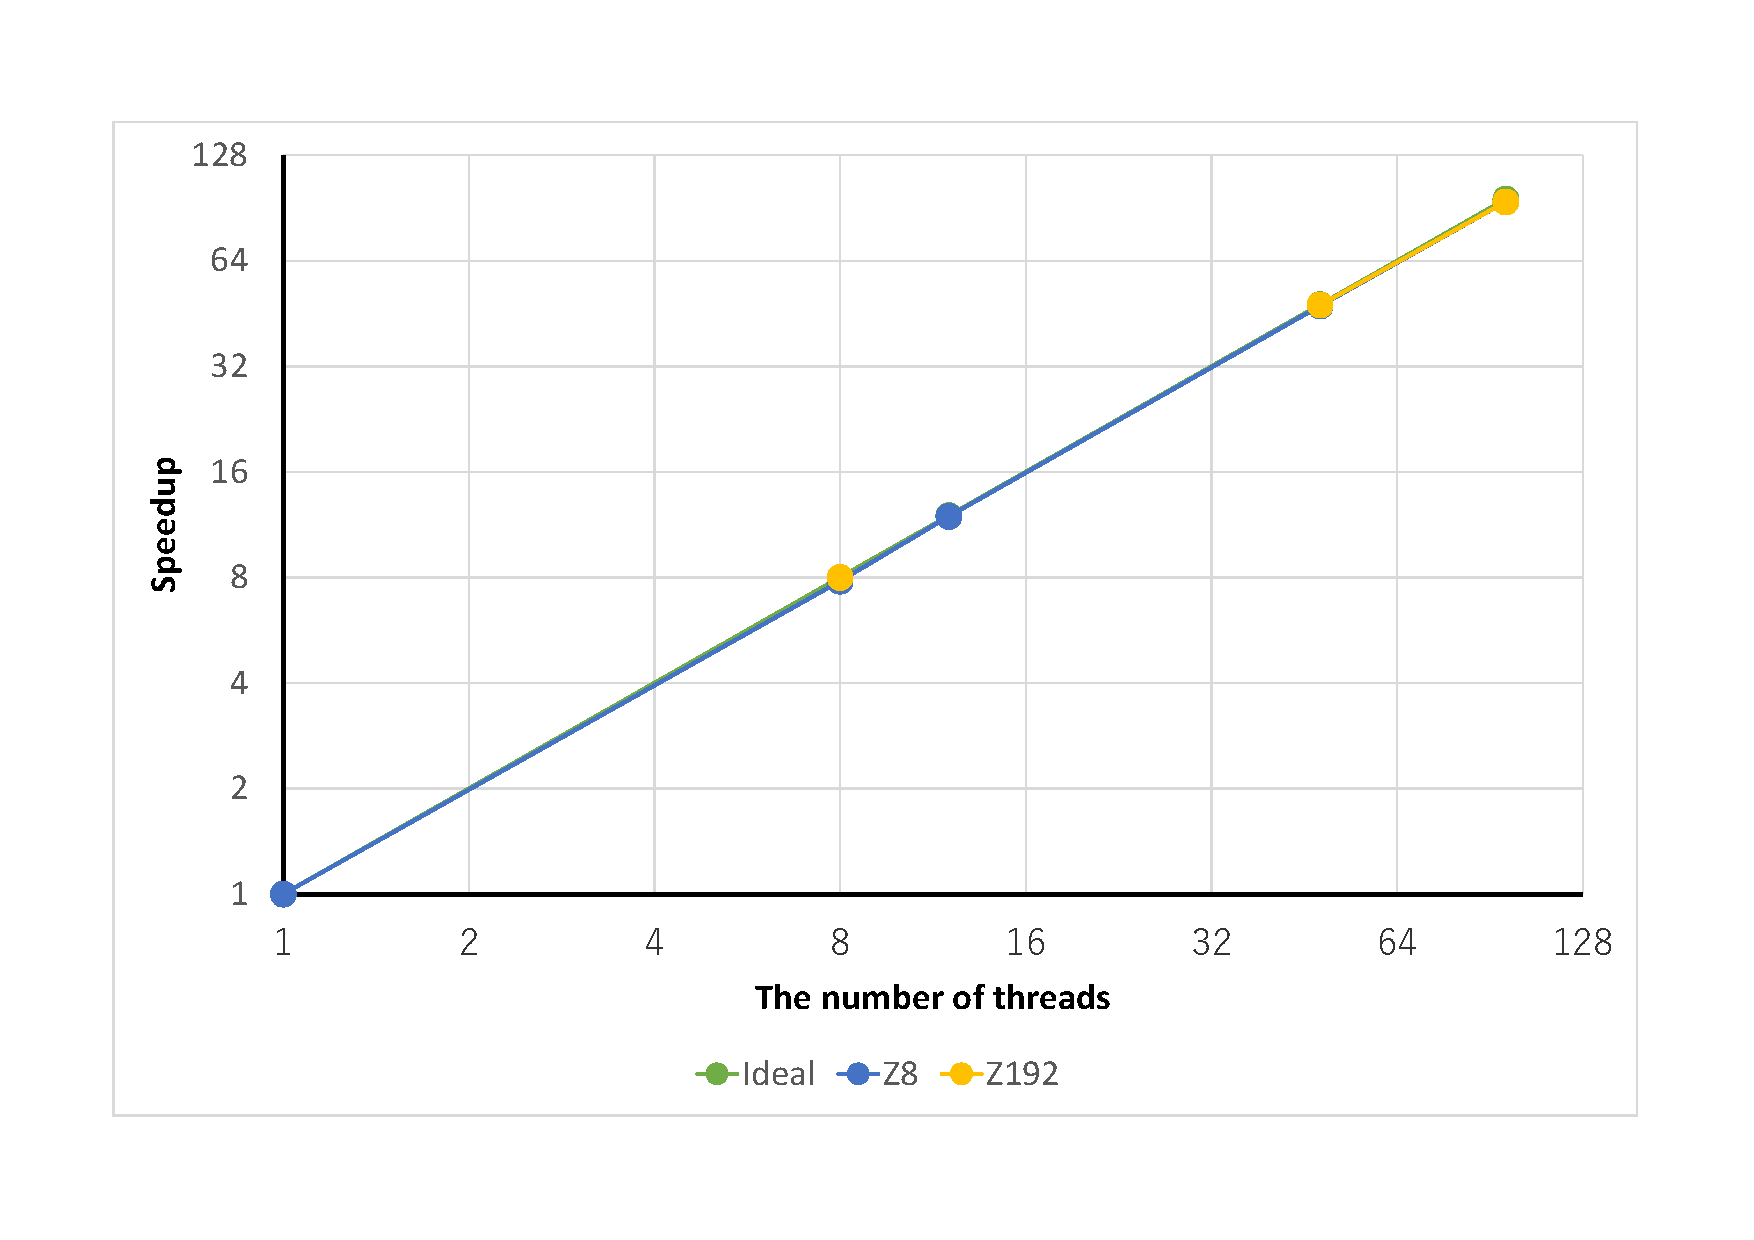
\includegraphics[width=10cm]{xmp96.pdf}
  \caption{The Speed-up ratio of Execution Parallelized by XcalableMP}\label{fig:xmp96}
  \end{center}
\end{figure}

\subsection{Comparison of Parallelization with MPI}

In order to compare the productivity of paralell programming, we also
implemented the reconstruction of three-dimensional atomic images with
MPI. The number of lines of the program in C already parallelized by
OpenMP is 350 and the number of modified or inserted lines for
multi-node parallelization by XcalableMP is 32, while that by MPI is
53. This program can be parallelized with smaller effort by XcalbleMP
than MPI.

Table \ref{tab:xmp_mpi} summerizes the execution time and the number
of modifed and inserted lines. The size of the reconstructed atomic
images is [z][x][y] = [192][192][192] and 96 threads are used in total
on the eight-node PC cluster. The difference of the execution time
parallelized by XcalableMP and MPI is small.
We confirmed that the higher productivity of parallel programming
is achieved by XcalableMP than MPI without sacrificing performance.

Data aggregation of the reconstructed atomic images
distributed among nodes is described by gmove statement
by XcalableMP, while called MPI\_Gatherv library function
by MPI. We comfirmed XcalableMP compiler transfers gmove
to appropriate MPI library functions.

\begin{table}[t]
  \begin{center}
    \caption{Execution Parallelized by XcalableMP and MPI
      (z:192, 96 threads)}\label{tab:xmp_mpi}
  \begin{tabular}{l|r|r}\hline\hline
    Parallelization & Time (s)  & \#modifed lines\\\hline\hline
    XcalableMP      & 1,840.942 & 32\\
    MPI             & 1,817.042 & 53\\
    \hline
  \end{tabular}
  \end{center}
\end{table}

\section{Conclusion}\label{sec:conclusion}

This chapter describes parallelization of reconstruction of
three-dimensional atomic images in X-ray fluorescence holography,
which is an analysis method of material science. In order to execute
it on large-scale PC clusters and supercomputer, we adopt hybrid
parallelization, or inter- and intra- node parallelization by
XcalableMP and OpenMP.

The program, whose input is 21 holograms data of 179 {$\times$} 360
points and output is a three-dimensional atomic image of {$192^3$}
points, is executed on PC cluster which consists of 8 nodes of Intel
Xeon X5660 processors and 96 cores in total, is executed in
1,841 seconds, or about half an hour. We estimated that it would take a
few days to execute this reconstruction sequentially. We confirmed
that the performance is improved by parallelization to the practical
use.

We also confirmed that the higher productivity of parallel programming
is achieved by XcalableMP than MPI without scrificing performance.

\begin{acknowledgement}
  The part of this work was supported by JSPS Grant-in-Aid for Scientific
  Research on Innovative Areas ``3D Activie-Site Science,`` Grant Number
  26105013.
\end{acknowledgement}
  
\bibliographystyle{spbasic}
\bibliography{xfh,parallel}
\end{document}
